\chapter{Metodologia}
\par O projeto será construído com base em uma residência modelo, que terá uma localização fixa e algumas restrições. O projeto modelo atenderá a uma residência de cinco pessoas e cômodos genéricos presentes nas casas tradicionais brasileiras, como quartos, cozinha, escritório, banheiros e área de serviço, podendo ser alterado de acordo com o desejo do cliente.
\par O sistema baseia-se em uma série de sensores interligados através da tecnologia smart grid e internet das coisas, gerando dados sobre o próprio funcionamento, consumo e utilização.  Esses dados serão interpretados e disponibilizados de forma simples porém compreensiva em um aplicativo de smartphone  para o cliente
\par Neste projeto, usaremos fontes alternativas de energia junto à energia da rede elétrica, e também outros meios possíveis (dependendo da casa) que contribuam com o meio ambiente, como reaproveitamento controlado da água, e com a eficiência energética da casa, garantindo um baixo custo operacional, além da economia ou até produção de energia.
\par A metodologia escolhida para o gerenciamento do projeto é a proposta pelo Project Management Institute - PMI, descrita na quinta edição do Guia PMBOK por conta do estilo do tema abordado, criando prazos e escolhas fixas, previamente acordadas para instalação do produto sem nenhum problema.
\par E para a organização das atividades utilizamos o conceito 5W2H, para facilitar o entendimento do projeto e agilizar a distribuição de atividade.
\par A sigla em língua inglesa 5W2H significa:
\begin{itemize}
    \item \textbf{What:} o que será feito;
    \item \textbf{Why:} por que será feito;
    \item \textbf{Where:} onde será feito;
    \item \textbf{When:} quando será feito;
    \item \textbf{Who:} por quem será feito;
    \item \textbf{How:} como será feito;
    \item \textbf{How much:} quanto vai custar.
\end{itemize}

\section{Grupos e Divisões}
\par A equipe foi dividida em  grupos específicos para cada atividade necessária. Cada grupo possui um gerente com o objetivo de facilitar a comunicação e atribuir as atividades referentes ao projeto.
\par \textbf{Gerência de Projeto:}
    \begin{itemize}
        \item Orientar a equipe, como um todo;
        \item Conferir e analisar o trabalho feito;
        \item Facilitar a comunicação entre os grupos;
        \item Coordenar as atividades.
    \end{itemize}
\par \textbf{Plataforma:}
    \begin{itemize}
        \item Seção de prototipagem;
        \item Seção de requisitos;
        \item Casos de uso do software;
        \item Pesquisa sobre IoT.
    \end{itemize}
\par \textbf{Sistema Energético:}
    \begin{itemize}
        \item Pesquisas sobre a parte energética residencial;
        \item Pesquisas sobre o Smart Grid;
        \item Pesquisa sobre fontes renováveis;
        \item Estudo sobre reaproveitamento da água.
    \end{itemize}
\par \textbf{Sistema de Automação:}
    \begin{itemize}
        \item Pesquisa sobre sensores;
        \item Pesquisa sobre atuadores;
        \item Pesquisa sobre central de comando.
    \end{itemize}
\par \textbf{Estudo da Casa:}
    \begin{itemize}
        \item Estudo da casa;
        \item Vida útil da tecnologia.
    \end{itemize}
\par \textbf{Edição e revisão de texto:}
    \begin{itemize}
        \item Ler e revisar tudo o que foi proposto, e tentar organizar o texto de maneira uniforme e compreensível.
    \end{itemize}
\par \textbf{Elaboração da Apresentação}
\par \textbf{Desenho técnico (CATIA)}

\section{Cronograma}
\par As atividades decorrem de acordo com nosso cronograma, atendendo o que foi proposto pela faculdade  e com validações de atividade, estando em mudança de acordo com as entregas de trabalho a até variações nas datas.
\par A especificação de cada proposta atividade é colocada nos documentos presentes na pasta compartilhada do Google Drive, e ao serem finalizadas, são imediatamente marcadas em verde no cronograma.

\begin{figure}[ht]
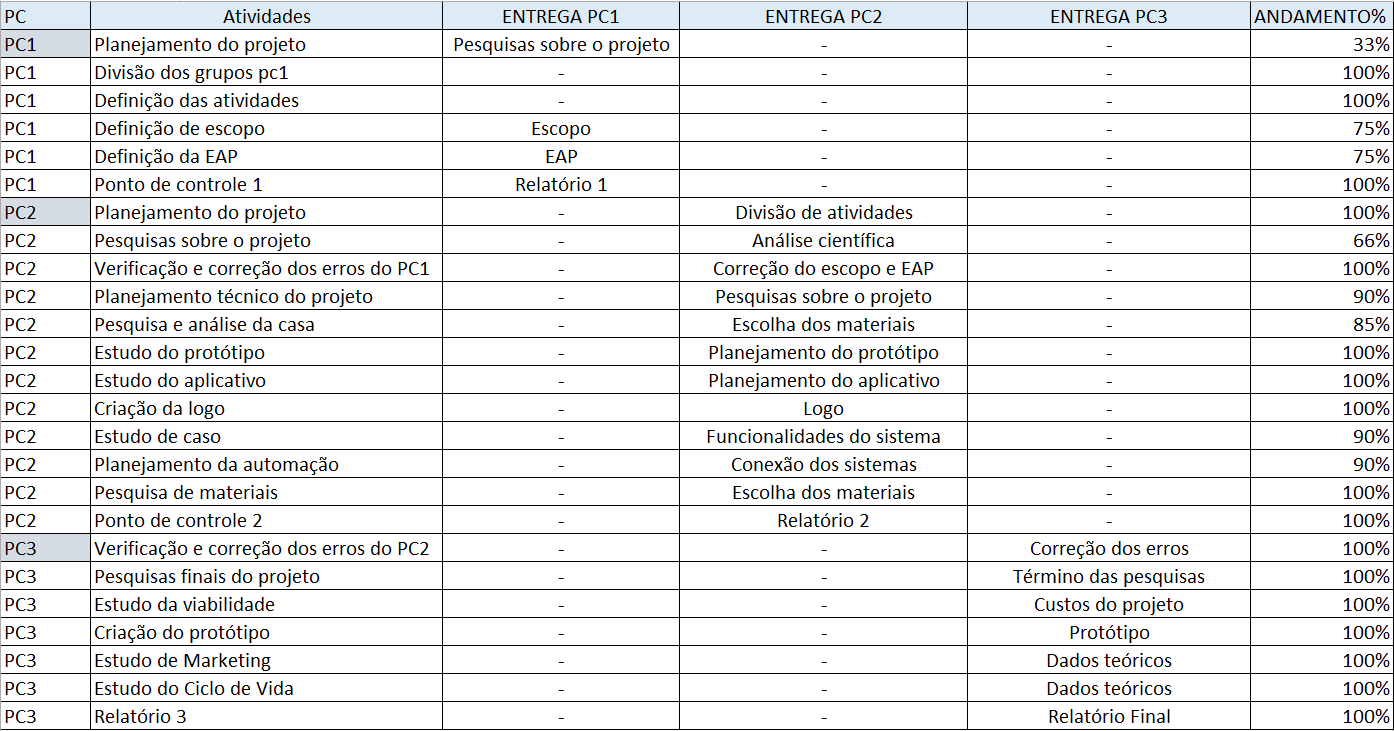
\includegraphics[width=\textwidth]{figuras/cronograma}
\end{figure}

\newpage

\section{Comunicação}
\par A equipe como um todo tem três meios de comunicação base, que envia as instruções como um todo para os integrantes. São elas:
\begin{itemize}
    \item Reuniões presenciais;
    \item WhatsApp;
    \item Slack.
\end{itemize}
\par As equipes têm livre escolha de quais mecanismos de comunicação serão por eles usadas. Em suas escolhas foram usados:
\begin{itemize}
    \item WhatsApp;
    \item Slack;
    \item Google Hangout;
    \item Discord.
\end{itemize}
